\documentclass[conference]{IEEEtran}
\usepackage[utf8]{inputenc}
\usepackage{amsmath,amssymb,graphicx,booktabs}

\usepackage[hidelinks,unicode,pdftitle={The Language-Modeling Cost Along the Base-to-Instruct Weight Interpolation Path of Qwen2.5-0.5B: WikiText-2 NLL versus ARC, HellaSwag and WinoGrande},pdfauthor={Dheiver Francisco Santos},pdfkeywords={weight interpolation, model merging, instruction tuning, perplexity, Qwen2.5},pdfsubject={Preprint, Figshare, doi:10.6084/m9.figshare.35014015}]{hyperref}
\begin{document}

\title{The Language-Modeling Cost Along the Base-to-Instruct Weight Interpolation Path of Qwen2.5-0.5B: WikiText-2 NLL versus ARC, HellaSwag and WinoGrande}

\author{\IEEEauthorblockN{Dheiver Francisco Santos, PhD}
\IEEEauthorblockA{Independent Researcher\\
Maceió, Alagoas, Brazil\\
ORCID: https://orcid.org/0000-0002-8599-9436\\
Preprint, Figshare, 2026, \href{https://doi.org/10.6084/m9.figshare.35014015}{doi:10.6084/m9.figshare.35014015}, CC BY 4.0}}

\maketitle

\begin{abstract}
Linear interpolation between a base language model and its instruction-tuned version, $\theta(t)=(1-t)\,\theta_{\text{base}}+t\,\theta_{\text{inst}}$, is often tuned for task accuracy alone. We measure what the same path does to language-modeling quality. For Qwen2.5-0.5B and its Instruct version, we evaluate 11 coefficients ($t=0,0.1,\dots,1$) on a macro-average of four multiple-choice benchmarks (3967 test items) and on WikiText-2 negative log-likelihood (NLL; 100 test blocks). All selection uses a disjoint validation split. The pre-registered hypothesis was that the accuracy-optimal $t^\ast$ differs from the NLL-optimal one. It holds only literally: validation picks $t^\ast_{\mathrm{NLL}}=0.1$ and $t^\ast_{\mathrm{acc}}=0.7$, but $t^\ast_{\mathrm{NLL}}=0.1$ is not distinguishable from the base (the interval contains zero) and $t^\ast_{\mathrm{acc}}=0.7$ rests on about one net validation item ($0.0008$). Test NLL rises from $t\approx0.2$ onward, reaching $+0.0886$ nats per token [$+0.0831$, $+0.0939$] at $t=1$. Accuracy shows no detectable difference from the base ($+0.65$ pp, 95\% CI $[-0.23,+1.52]$). Evaluation in bfloat16 agrees with fp32 to within 0.003 nats. The study covers one model pair, one scale and one path.
\end{abstract}

\begin{IEEEkeywords}
weight interpolation, model merging, instruction tuning, perplexity, Qwen2.5
\end{IEEEkeywords}

\section{Introduction}
Interpolating the weights of a pre-trained model and its fine-tuned descendant is a cheap way to trade one behavior for another. The path has one scalar, $t$, and every point on it costs one forward pass of evaluation. Practitioners usually select $t$ for the benchmark of interest. Instruction tuning, however, changes the model's output distribution, so the coefficient that is best for multiple-choice accuracy need not be best for modeling raw text.

This paper asks one question: along the base$\leftrightarrow$instruct path of Qwen2.5-0.5B \cite{qwen25}, does the coefficient that maximizes validation accuracy differ from the coefficient that minimizes validation WikiText-2 NLL, and how large is the measured cost of moving between them? A pre-registration fixed the question, the grid and the accuracy metrics before any model was merged (hypothesis 10); for NLL it fixed only the WikiText-2 NLL, and the split into validation blocks 0--39 and test blocks 40--139 is recorded in \texttt{results/FACTS.md}. Selection used only validation items and blocks, and the test split was read once per configuration.

Contributions: (i) a paired, block-level measurement of the NLL cost along the whole path, with the accuracy curve evaluated on the same models; (ii) the observation that the validation-optimal accuracy coefficient is weakly identified, since validation accuracy varies by about one percentage point or less across the path; and (iii) a plain statement of what a correlation over 11 dependent points can and cannot say.

\section{Related Work}
\textbf{Interpolating and averaging weights.} Interpolation between a zero-shot model and its fine-tuned version improves robustness under distribution shift in WiSE-FT \cite{wortsman2021wiseft}, and averaging many fine-tuned models gives model soups \cite{wortsman2022soups}. Model Ratatouille recycles diverse fine-tunings of the same pre-trained model to improve out-of-distribution generalization \cite{rame2022ratatouille}. They target classification accuracy or robustness, not language modeling.

\textbf{Trade-offs and Pareto fronts.} Rewarded soups interpolate weights fine-tuned on different rewards and trace a Pareto front between the rewards \cite{rame2023rewardedsoups}. Our setting has two metrics, accuracy and perplexity, on the path between one pair of endpoints; we report both curves but do not analyze a Pareto front. Chat Vector adds the difference between a chat model and its base to another model, extending instruction following across languages \cite{huang2023chatvector}; the same difference, scaled by $t$, is the path measured here. Task arithmetic gives the general view in which such differences are editable directions \cite{ilharco2022taskarith,ortizjimenez2023tangent}.

\textbf{When interpolation is well behaved.} Interpolation between networks avoids a loss barrier when they are linearly mode connected \cite{frankle2019lmc}; TIES resolves interference between task vectors \cite{yadav2023ties}, and Fisher weighting weights parameters by their estimated importance \cite{matena2021fisher}, and recent work examines merging at scale \cite{yadav2024scale}. Surveys summarize the field \cite{yang2024mergingsurvey}.

\textbf{Evaluation.} We score multiple-choice tasks by log-likelihood \cite{gao2021lmeval} on ARC \cite{clark2018arc}, HellaSwag \cite{zellers2019hellaswag} and WinoGrande \cite{sakaguchi2019winogrande}, and language modeling on WikiText-2 \cite{merity2016pointer}. Statistical reporting follows paired-difference practice \cite{miller2024errorbars} and the bootstrap \cite{efron1979bootstrap}; selecting on one split and reporting on another follows standard practice, although reusing a holdout adaptively can still bias estimates \cite{dwork2014adaptive}. We did not find a systematic measurement of the raw-text perplexity cost as a function of the interpolation coefficient on a base/instruct pair with block-paired intervals; this paper provides one.

\textbf{Author's related work.} The author's technical notes cover neighboring topics in language-model training: model merging for capability composition \cite{santos2026modelmergingfo}, direct preference optimization \cite{santos2026directpreferen}, knowledge distillation and self-distillation \cite{santos2026knowledgedisti}, parameter-efficient fine-tuning (LoRA, QLoRA, DoRA) \cite{santos2026parametereffic}, mixture-of-experts training and sparse upcycling \cite{santos2026mixtureofexper}, curriculum learning and data-efficient pretraining \cite{santos2026curriculumlear}, synthetic data generation and self-improvement \cite{santos2026syntheticdatag}, and RLAIF and Constitutional AI \cite{santos2026rlaifandconsti}. This paper instead reports a controlled held-out measurement. In a different domain, the author's JEPA preprint \cite{santos2026collapseresist} uses a similar controlled-comparison style (identical budgets, several seeds, confidence intervals).

\section{Method}
Let $\theta_{\text{base}}$ and $\theta_{\text{inst}}$ be the weights of Qwen2.5-0.5B and Qwen2.5-0.5B-Instruct (same architecture). For $t\in\{0,0.1,\dots,1\}$,
\begin{equation}
\theta(t)=(1-t)\,\theta_{\text{base}}+t\,\theta_{\text{inst}},
\end{equation}
computed per tensor in fp32 and copied to the model.

\subsection*{Equations and their meaning}
Eq.~(1) is a straight line in weight space: $t=0$ is the base model, $t=1$ is the instruct model, and $t=0.5$ is the midpoint. Equivalently $\theta(t)=\theta_{\text{base}}+t\,(\theta_{\text{inst}}-\theta_{\text{base}})$, i.e.\ the instruction-tuning difference scaled by $t$.

The accuracy metric is the macro-average over the four tasks $\mathcal{T}$,
\begin{equation}
A(t)=\frac{1}{|\mathcal{T}|}\sum_{\tau\in\mathcal{T}}\frac{1}{n_\tau}\sum_{i=1}^{n_\tau} y_{\tau i}(t),
\end{equation}
where $y_{\tau i}(t)\in\{0,1\}$ is 1 if the model scores the correct answer highest by log-likelihood on item $i$ of task $\tau$. Every task counts equally regardless of its size.

The language-modeling metric is the mean per-block NLL over a set $\mathcal{B}$ of blocks of $L=512$ tokens,
\begin{equation}
N(t)=\frac{1}{|\mathcal{B}|}\sum_{b\in\mathcal{B}}\ell_b(t),\quad \ell_b(t)=-\frac{1}{L}\sum_{i=1}^{L}\log p_{\theta(t)}(x_{i+1}\mid x_{\le i}),
\end{equation}
the average negative log-probability per token, in nats. Lower is better and $e^{N}$ is perplexity.

The selected coefficients on validation are
\begin{equation}
t^\ast_{\mathrm{acc}}=\arg\max_t A_{\mathrm{val}}(t),\qquad t^\ast_{\mathrm{NLL}}=\arg\min_t N_{\mathrm{val}}(t),
\end{equation}
and the hypothesis is $t^\ast_{\mathrm{acc}}\neq t^\ast_{\mathrm{NLL}}$. The cost of a coefficient is the paired difference
\begin{equation}
C(t)=\frac{1}{|\mathcal{B}_{\mathrm{test}}|}\sum_{b}\big[\ell_b(t)-\ell_b(0)\big],
\end{equation}
positive when the interpolated model models text worse than the base. Finally, the descriptive association over the 11 grid points is the Pearson correlation $r=\mathrm{corr}\big(A_{\mathrm{test}}(t),N_{\mathrm{test}}(t)\big)$; a positive $r$ means that higher accuracy goes with higher (worse) NLL.

\section{Experimental Protocol}
\textbf{Models.} Qwen2.5-0.5B (base) and Qwen2.5-0.5B-Instruct, both Apache-2.0, at Hub revisions \texttt{060db649} and \texttt{7ae55760} (full hashes in \texttt{MANIFEST.json}) \cite{qwen25}. Evaluation in bfloat16 on Apple Silicon (MPS), PyTorch 2.8.0, transformers 4.57.6; interpolation in fp32 on CPU. There is no training and the evaluation is deterministic; there are no random seeds, and the bootstrap seed is 0.

\textbf{Data and splits.} Accuracy: ARC-Easy, ARC-Challenge, HellaSwag (length-normalized by characters) and WinoGrande (partial scoring, no normalization). Validation uses 300 items per task (299 for ARC-Challenge) and test 1000 per task (967 for WinoGrande), 3967 test items; splits are disjoint (seed 0). ARC uses its official validation and test splits; HellaSwag and WinoGrande items come from their validation sets, partitioned into validation and test. Language modeling: the WikiText-2 test text is tokenized with the Qwen tokenizer and cut into consecutive 512-token blocks; blocks $0$--$39$ are validation and $40$--$139$ are test (100 test blocks).

\textbf{Selection.} Hypothesis 10 (pre-registered): $t^\ast_{\mathrm{acc}}$ differs from $t^\ast_{\mathrm{NLL}}$ along the Qwen base$\leftrightarrow$instruct path, grid $t=0,0.1,\dots,1$. Both optima are chosen on validation only (accuracy on 1199 validation items, NLL on 40 blocks), and the test split is used only to report each configuration. The comparison point for gains is the base model ($t=0$), the best original model on validation accuracy. This is a secondary measurement built on the accuracy grid of the companion LERP experiment (same models, same grid, same items).

\textbf{Baselines.} Base ($t=0$) and instruct ($t=1$) are the two original models; the interpolated points are never compared with an oracle chosen on test data.

\textbf{Statistics.} Accuracy: bootstrap over items (2000 resamples for one accuracy, 3000 for paired differences), macro-averaged with tasks equally weighted, 95\% percentile CI. NLL: paired bootstrap over test blocks (5000 resamples), 95\% CI of $C(t)$. The 100 blocks are consecutive text and not independent draws, so the NLL intervals describe variation across these blocks. The correlation $r$ is computed over 11 points along one path (adjacent points share almost all weights), so it is descriptive and has no inferential interpretation; we give no $p$ for it. The ten NLL comparisons against the base ($t=0.1,\dots,1.0$) are not corrected for multiplicity. At 99.5\% (Bonferroni level for ten comparisons), the interval at $t=0.2$ becomes $[-0.0002,+0.0033]$ and includes zero (\texttt{results/ci995\_art10.txt}), so the onset at $t=0.2$ is not robust; $t=0.3$ stays above zero. The accuracy comparison against the base at $t^\ast_{\mathrm{acc}}$ has nominal $p=0.149$. The pre-registration (\texttt{experiments/PREREG.md}) fixed 5,000 resamples. The analysis deviated for accuracy: the paired difference at $t=0.7$ uses 3000 (\texttt{analyze.py}), and the one at $t=1$ uses 5000 (\texttt{experiments/extra\_art07\_art10.py}).

\section{Results}
Table~\ref{tab:frontier} lists, for every $t$, validation and test NLL, the paired NLL cost relative to the base on test blocks, and macro accuracy on validation and test (bootstrap CI over items).

\begin{table*}[!t]
\caption{Qwen2.5-0.5B base$\leftrightarrow$instruct path. NLL in nats per token on WikiText-2 (validation: 40 blocks; test: 100 blocks); $C(t)$ is the paired test-block difference from $t=0$ with 95\% bootstrap CI. Accuracy: macro-average of four tasks (validation $n=1199$, test $n=3967$), 95\% bootstrap CI over items.}
\label{tab:frontier}
\centering
\small
\begin{tabular}{crrrcc}
\toprule
$t$ & Val NLL & Test NLL & $C(t)$ [95\% CI] & Val acc. & Test acc. [95\% CI] \\
\midrule
0.0 & 2.8051 & 2.8533 & --- & 0.4953 & 0.5025 [0.4875, 0.5174] \\
0.1 & 2.8047 & 2.8525 & $-0.0008$ [$-0.0018$, $+0.0001$] & 0.4928 & 0.5020 [0.4863, 0.5171] \\
0.2 & 2.8072 & 2.8549 & $+0.0016$ [$+0.0004$, $+0.0028$] & 0.4945 & 0.4983 [0.4831, 0.5135] \\
0.3 & 2.8095 & 2.8584 & $+0.0051$ [$+0.0036$, $+0.0066$] & 0.4953 & 0.5001 [0.4844, 0.5150] \\
0.4 & 2.8147 & 2.8649 & $+0.0115$ [$+0.0097$, $+0.0135$] & 0.4953 & 0.5029 [0.4874, 0.5183] \\
0.5 & 2.8225 & 2.8719 & $+0.0185$ [$+0.0162$, $+0.0209$] & 0.4936 & 0.5021 [0.4869, 0.5174] \\
0.6 & 2.8335 & 2.8823 & $+0.0289$ [$+0.0258$, $+0.0319$] & 0.4853 & 0.5087 [0.4940, 0.5241] \\
0.7 & 2.8446 & 2.8932 & $+0.0398$ [$+0.0364$, $+0.0432$] & 0.4961 & 0.5090 [0.4938, 0.5246] \\
0.8 & 2.8582 & 2.9057 & $+0.0524$ [$+0.0483$, $+0.0564$] & 0.4953 & 0.5074 [0.4920, 0.5226] \\
0.9 & 2.8750 & 2.9219 & $+0.0686$ [$+0.0640$, $+0.0729$] & 0.4928 & 0.5083 [0.4929, 0.5241] \\
1.0 & 2.8972 & 2.9419 & $+0.0886$ [$+0.0831$, $+0.0939$] & 0.4853 & 0.5064 [0.4909, 0.5220] \\
\bottomrule
\end{tabular}
\end{table*}

\begin{figure}[!t]
\centering
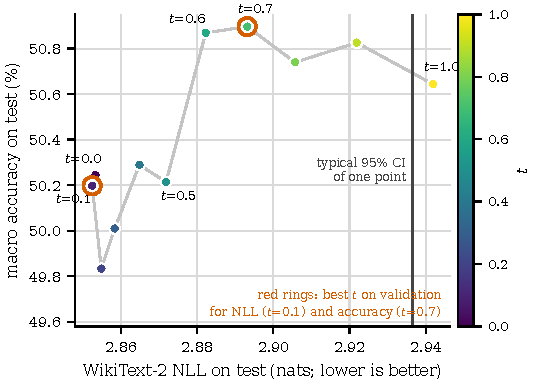
\includegraphics[width=\columnwidth]{figs/fig10_frontier.pdf}
\caption{Test macro accuracy versus test WikiText-2 NLL along the path, one point per $t$ (color). Red rings mark the validation-best $t$ for NLL and for accuracy; the reference bar is a typical 95\% CI of one point. NLL rises while accuracy stays within noise. Pearson $r=0.740$ (descriptive; points are dependent).}
\label{fig:frontier}
\end{figure}

\textbf{Pre-registered hypothesis.} The two selected coefficients differ: $t^\ast_{\mathrm{NLL}}=0.1$ and $t^\ast_{\mathrm{acc}}=0.7$ on validation. This holds only literally, and the two optima are not equally well determined. Validation NLL at $t=0$ and $t=0.1$ differs by $0.0004$ nats, and the test difference is $-0.0008$ [$-0.0018$, $+0.0001$], which includes zero. So $t^\ast_{\mathrm{NLL}}=0.1$ is not distinguishable from the base. Validation accuracy ranges only from $0.4853$ to $0.4961$ over the 11 points. There $t^\ast_{\mathrm{acc}}=0.7$ (0.4961) beats $t=0$ (0.4953) by $0.0008$, one net item out of 1199 ($1/1200\approx0.0008$). A test accuracy has a bootstrap CI of the order of $\pm1.5$ pp, so the validation argmax is determined largely by noise. The distinct optima therefore reflect a flat accuracy curve and a rising NLL curve rather than two sharply located peaks.

\textbf{Cost in language modeling.} NLL on test blocks is within noise of the base up to $t=0.1$, then rises monotonically in $t$ in the table: $+0.0185$ [$+0.0162$, $+0.0209$] at $t=0.5$, $+0.0398$ [$+0.0364$, $+0.0432$] at $t=0.7$, and $+0.0886$ [$+0.0831$, $+0.0939$] at $t=1$. All intervals from $t=0.2$ on lie above zero. In perplexity units, computed from the mean NLL, $t=0$ gives about $17.3$ and $t=1$ about $19.0$ on these 100 blocks, i.e.\ about $9\%$ higher.

\textbf{Accuracy along the path.} At the validation-selected $t^\ast_{\mathrm{acc}}=0.7$ the test accuracy is $0.5090$ [$0.4938$, $0.5246$] against $0.5025$ for the base: a paired difference of $+0.65$ pp [$-0.23$, $+1.52$], $p=0.149$, which shows no difference detected (no equivalence test). The instruct endpoint is $+0.40$ pp [$-0.62$, $+1.40$] over the base on the paired macro accuracy. The point estimates are higher at $t\ge0.6$ than at $t\le0.5$ ($0.5064$--$0.5090$ versus $0.4983$--$0.5029$), but the intervals overlap throughout, so we do not claim an accuracy gain.

\textbf{Correlation.} Over the 11 points, test accuracy and test NLL have Pearson $r=0.740$: points with higher accuracy tend to have higher NLL. Because the points lie on one path and adjacent coefficients share nearly the same weights, $r$ does not support a sampling-based statement; it summarizes the shape of the curves in Fig.~\ref{fig:frontier}. Its sign only says that the accuracy point estimates and the NLL rise together; it is not a Pareto analysis.

\textbf{Reading the result.} The data give two measurements. The NLL cost is estimated: $+0.0398$ nats [$+0.0364$, $+0.0432$] at $t=0.7$ and $+0.0886$ [$+0.0831$, $+0.0939$] at $t=1$. An accuracy gain is not detected: at $t=0.7$ the upper end of the 95\% CI is $+1.52$ pp, and at $t=1$ it is $+1.40$ pp. Gains up to those bounds cannot be excluded, and none is shown.

\section{Discussion and Limitations}
\textbf{Numerical precision.} All models were evaluated in bfloat16. We repeated the NLL evaluation in fp32 for all 11 coefficients and the validation accuracy for $t=0$, $0.7$ and $1$ (Table~\ref{tab:fp32}; \texttt{experiments/an\_art10\_fp32.py}, \texttt{results/summary\_art10\_fp32.txt}, \texttt{results/fp32\_check\_qwen.txt}). The bf16$-$fp32 difference of the test NLL lies in $[-0.0001,+0.0025]$ over the 11 coefficients (validation: at most $+0.0026$). The fp32 test cost at $t=1$ is $+0.0877$ nats, against $+0.0886$ in bf16. The validation NLL minimum in fp32 is at $t=0$ ($2.8032$), not at $t=0.1$ ($2.8037$): the two differ by $0.0005$ nats, so $t^\ast_{\mathrm{NLL}}=0.1$ depends on the precision and is poorly determined; no interval was computed for this gap. Validation macro accuracy in fp32 is $0.4886$, $0.4920$ and $0.4845$ at $t=0$, $0.7$ and $1$ (bf16: $0.4953$, $0.4961$, $0.4853$). The order of the three is the same, and the fp32 gap between $t=0.7$ and $t=0$ ($+0.0034$) is of the order of 4 items, and no interval was computed for fp32. The size of the NLL cost and the absence of a detected accuracy gain do not change.

\begin{table}[!t]
\caption{Precision sensitivity: mean NLL (nats per token), bf16 versus fp32, at three coefficients, and the validation macro accuracy in bf16 and fp32.}
\label{tab:fp32}
\centering
\footnotesize\setlength{\tabcolsep}{3pt}
\begin{tabular}{crrrrrr}
\toprule
$t$ & \multicolumn{2}{c}{Val NLL} & \multicolumn{2}{c}{Test NLL} & \multicolumn{2}{c}{Val acc.} \\
& bf16 & fp32 & bf16 & fp32 & bf16 & fp32 \\
\midrule
0.0 & 2.8051 & 2.8032 & 2.8533 & 2.8517 & 0.4953 & 0.4886 \\
0.1 & 2.8047 & 2.8037 & 2.8525 & 2.8526 & --- & --- \\
0.7 & 2.8446 & 2.8429 & 2.8932 & 2.8912 & 0.4961 & 0.4920 \\
1.0 & 2.8972 & 2.8947 & 2.9419 & 2.9394 & 0.4853 & 0.4845 \\
\bottomrule
\end{tabular}
\end{table}

\textbf{What we conjecture.} We conjecture that the NLL cost reflects the shift of the output distribution toward the instruction-tuning data and away from raw web and encyclopedic text; this is an interpretation and was not tested (no probing of the tuning data, no per-token analysis, no control with a different tuned model). The measured fact is the cost curve and its size.

\textbf{Threats to validity.} (i) One model pair, one scale (0.5B), one hardware and one path; other tuned models, scales or interpolation operations may differ. (ii) The accuracy effect is within noise, so the result is better read as ``NLL cost measured, accuracy benefit not detected'' than as a balance between two measured effects. (iii) NLL is measured on one corpus with 100 consecutive blocks; WikiText-2 is encyclopedic text, and the cost may differ on other text. (iv) The validation and test blocks are adjacent stretches of the same corpus. (v) We did not check either model for contamination of the benchmarks or of WikiText-2. (vi) The correlation uses 11 dependent points, and no inference is attached. (vii) We did not evaluate generation quality or instruction following, which an instruction-tuned model is meant to improve. A perplexity cost can be acceptable for a user who wants those. (viii) The tasks are knowledge and common-sense multiple-choice benchmarks scored by log-likelihood, the regime in which a base model is already strong.

\textbf{Use.} A practitioner who selects $t$ by accuracy alone on these benchmarks will not detect a gain and will pay a measurable perplexity cost when $t$ is large. A small $t$ ($\le0.1$) costs nothing detectable in NLL. Whether an interior $t$ is worth its cost depends on a downstream objective that this study does not measure.

\section{Conclusion}
Along the Qwen2.5-0.5B base$\leftrightarrow$instruct interpolation path, the validation-optimal coefficient for accuracy ($0.7$) differs from that for WikiText-2 NLL ($0.1$), confirming the pre-registered hypothesis in the literal sense. Test NLL rises with $t$ from about $0.2$--$0.3$ on (the $t=0.2$ onset is not robust to multiplicity), to $+0.0886$ nats [$+0.0831$, $+0.0939$] at $t=1$, while accuracy shows no detectable difference from the base ($+0.65$ pp [$-0.23$, $+1.52$] at $t=0.7$). Test accuracy and NLL correlate at $r=0.740$ over the 11 dependent points, a descriptive summary of the curve shapes. In fp32 the validation NLL minimum moves to $t=0$, not distinguishable from $t=0.1$. The result comes from one pair, one scale and one corpus. Whether an accuracy gain exists, or pays for the cost, is not settled here.

\section*{Data and Code Availability}
All code, per-item caches and summaries are in the repository \texttt{artigos-pesos-modelos-pequenos} at git tag \texttt{preprints-v1} (the commit that contains this manuscript and all scripts and caches); the pre-registration is \texttt{experiments/PREREG.md} (written before any merge). Numbers come from \texttt{results/summary\_art10.txt}, \texttt{results/summary\_art01.txt} (accuracy) and \texttt{results/extra\_art07\_art10.txt} (per-$t$ NLL differences and the paired accuracy at $t=1$, script \texttt{experiments/extra\_art07\_art10.py}) and \texttt{results/summary\_art10\_fp32.txt} (precision check, script \texttt{experiments/an\_art10\_fp32.py}). One command regenerates tables and figure: \texttt{./run\_everything.sh}. Versions: Python 3.9.6, PyTorch 2.8.0, transformers 4.57.6, numpy 1.26.4, datasets 4.5.0. Model revisions: Qwen2.5-0.5B \texttt{060db6499f32faf8b98477b0a26969ef7d8b9987}, Qwen2.5-0.5B-Instruct \texttt{7ae557604adf67be50417f59c2c2f167def9a775}. Evaluation is deterministic; the bootstrap seed is 0.

\section*{Acknowledgments}
No external funding.

\begin{thebibliography}{99}
\bibitem{qwen25} Qwen Team, A. Yang, B. Yang, et al., ``Qwen2.5 technical report,'' arXiv:2412.15115, 2024.
\bibitem{wortsman2021wiseft} M. Wortsman, G. Ilharco, J. W. Kim, et al., ``Robust fine-tuning of zero-shot models,'' in \emph{Proc.\ CVPR}, 2022, arXiv:2109.01903.
\bibitem{wortsman2022soups} M. Wortsman, G. Ilharco, S. Y. Gadre, et al., ``Model soups: Averaging weights of multiple fine-tuned models improves accuracy without increasing inference time,'' in \emph{Proc.\ ICML}, 2022, arXiv:2203.05482.
\bibitem{rame2022ratatouille} A. Ram\'e, K. Ahuja, J. Zhang, M. Cord, et al., ``Model Ratatouille: Recycling diverse models for out-of-distribution generalization,'' in \emph{Proc.\ ICML}, 2023, arXiv:2212.10445.
\bibitem{rame2023rewardedsoups} A. Ram\'e, G. Couairon, M. Shukor, C. Dancette, et al., ``Rewarded soups: Towards Pareto-optimal alignment by interpolating weights fine-tuned on diverse rewards,'' in \emph{Proc.\ NeurIPS}, 2023, arXiv:2306.04488.
\bibitem{huang2023chatvector} S.-C. Huang, P.-Z. Li, Y.-C. Hsu, K.-M. Chen, et al., ``Chat Vector: A simple approach to equip LLMs with instruction following and model alignment in new languages,'' in \emph{Proc.\ ACL}, 2024, arXiv:2310.04799.
\bibitem{ilharco2022taskarith} G. Ilharco, M. T. Ribeiro, M. Wortsman, et al., ``Editing models with task arithmetic,'' in \emph{Proc.\ ICLR}, 2023, arXiv:2212.04089.
\bibitem{ortizjimenez2023tangent} G. Ortiz-Jimenez, A. Favero, and P. Frossard, ``Task arithmetic in the tangent space: Improved editing of pre-trained models,'' in \emph{Proc.\ NeurIPS}, 2023, arXiv:2305.12827.
\bibitem{frankle2019lmc} J. Frankle, G. K. Dziugaite, D. M. Roy, and M. Carbin, ``Linear mode connectivity and the lottery ticket hypothesis,'' in \emph{Proc.\ ICML}, 2020, arXiv:1912.05671.
\bibitem{matena2021fisher} M. Matena and C. Raffel, ``Merging models with Fisher-weighted averaging,'' in \emph{Proc.\ NeurIPS}, 2022, arXiv:2111.09832.
\bibitem{yadav2023ties} P. Yadav, D. Tam, L. Choshen, et al., ``TIES-Merging: Resolving interference when merging models,'' in \emph{Proc.\ NeurIPS}, 2023, arXiv:2306.01708.
\bibitem{yadav2024scale} P. Yadav, T. Vu, J. Lai, et al., ``What matters for model merging at scale?'' arXiv:2410.03617, 2024.
\bibitem{yang2024mergingsurvey} E. Yang, L. Shen, G. Guo, et al., ``Model merging in LLMs, MLLMs, and beyond: Methods, theories, applications and opportunities,'' arXiv:2408.07666, 2024.
\bibitem{gao2021lmeval} L. Gao et al., ``EleutherAI/lm-evaluation-harness,'' Zenodo, doi:10.5281/zenodo.10256836.
\bibitem{clark2018arc} P. Clark, I. Cowhey, O. Etzioni, T. Khot, et al., ``Think you have solved question answering? Try ARC, the AI2 reasoning challenge,'' arXiv:1803.05457, 2018.
\bibitem{zellers2019hellaswag} R. Zellers, A. Holtzman, Y. Bisk, A. Farhadi, and Y. Choi, ``HellaSwag: Can a machine really finish your sentence?'' in \emph{Proc.\ ACL}, 2019, arXiv:1905.07830.
\bibitem{sakaguchi2019winogrande} K. Sakaguchi, R. Le Bras, C. Bhagavatula, and Y. Choi, ``WinoGrande: An adversarial Winograd schema challenge at scale,'' in \emph{Proc.\ AAAI}, 2020, arXiv:1907.10641.
\bibitem{merity2016pointer} S. Merity, C. Xiong, J. Bradbury, and R. Socher, ``Pointer sentinel mixture models,'' in \emph{Proc.\ ICLR}, 2017, arXiv:1609.07843.
\bibitem{miller2024errorbars} E. Miller, ``Adding error bars to evals: A statistical approach to language model evaluations,'' arXiv:2411.00640, 2024.
\bibitem{efron1979bootstrap} B. Efron, ``Bootstrap methods: Another look at the jackknife,'' \emph{Ann.\ Statist.}, vol.~7, no.~1, pp.~1--26, 1979, doi:10.1214/aos/1176344552.
\bibitem{dwork2014adaptive} C. Dwork, V. Feldman, M. Hardt, T. Pitassi, et al., ``Preserving statistical validity in adaptive data analysis,'' in \emph{Proc.\ STOC}, 2015, arXiv:1411.2664.
\bibitem{santos2026modelmergingfo} D. F. Santos, ``Model Merging for Capability Composition: A Technical Note,'' Zenodo, 2026, doi:10.5281/zenodo.21610555.
\bibitem{santos2026collapseresist} D. F. Santos, ``Collapse-Resistant Joint-Embedding Predictive Architectures: A Controlled Comparison of SIGReg, VICReg, and EMA,'' Zenodo, v2, 2026, doi:10.5281/zenodo.24223364.
\bibitem{santos2026directpreferen} D. F. Santos, ``Direct Preference Optimization (DPO): A Technical Note,'' Zenodo, 2026, doi:10.5281/zenodo.21609911.
\bibitem{santos2026knowledgedisti} D. F. Santos, ``Knowledge Distillation and Self-Distillation for Language Models,'' Zenodo, 2026, doi:10.5281/zenodo.21610100.
\bibitem{santos2026parametereffic} D. F. Santos, ``Parameter-Efficient Fine-Tuning: LoRA, QLoRA, and DoRA,'' Zenodo, 2026, doi:10.5281/zenodo.21610033.
\bibitem{santos2026mixtureofexper} D. F. Santos, ``Mixture-of-Experts Training and Sparse Upcycling,'' Zenodo, 2026, doi:10.5281/zenodo.21610062.
\bibitem{santos2026curriculumlear} D. F. Santos, ``Curriculum Learning and Data-Efficient Pretraining: A Technical Note,'' Zenodo, 2026, doi:10.5281/zenodo.21610595.
\bibitem{santos2026syntheticdatag} D. F. Santos, ``Synthetic Data Generation and Self-Improvement: A Technical Note,'' Zenodo, 2026, doi:10.5281/zenodo.21610525.
\bibitem{santos2026rlaifandconsti} D. F. Santos, ``RLAIF and Constitutional AI: A Technical Note,'' Zenodo, 2026, doi:10.5281/zenodo.21610280.
\end{thebibliography}

\end{document}
